\chapter{Graph}

\section{Alien Dictionary} %%%%%%%%%%%%%%%%%%%%%%

\subsubsection{Description}
There is a new alien language which uses the latin alphabet. However, the order among letters are unknown to you. You receive a list of non-empty words from the dictionary, where words are sorted lexicographically by the rules of this new language. Derive the order of letters in this language.

\textbf{Example:}

Given the following words in dictionary,
\begin{Code}
[
  "wrt",
  "wrf",
  "er",
  "ett",
  "rftt"
]
\end{Code}

The correct order is: \code{"wertf"}.

\textbf{Note:}

1. You may assume all letters are in lowercase.

2. You may assume that if a is a prefix of b, then a must appear before b in the given dictionary.

3. If the order is invalid, return an empty string.

4. There may be multiple valid order of letters, return any one of them is fine.

\newpage

\subsubsection{Solution}

\begin{Code}
public String alienOrder(String[] words) {
    int[] indegree = new int[26];
    Arrays.fill(indegree, -1);

    int count = 0;
    for (String word : words) {
        for (char c : word.toCharArray()) {
            if (indegree[c - 'a'] != 0) {
                indegree[c - 'a'] = 0;
                count++;
            }
        }
    }
    HashMap<Character, Set<Character>> map = new HashMap<>();
    for (int i = 0; i < words.length - 1; i++) {
        String first = words[i], second = words[i + 1];
        int len = Math.min(first.length(), second.length());
        for (int j = 0; j < len; j++) {
            if (first.charAt(j) != second.charAt(j)) {
                Set<Character> set = map.get(first.charAt(j));
                if (set == null) {
                    set = new HashSet<Character>();
                    map.put(first.charAt(j), set);
                }
                if (set.add(second.charAt(j))) {
                    indegree[second.charAt(j) - 'a']++;
                }
                break;
            } else {
                if (j + 1 >= second.length() && j + 1 < first.length()) { return ""; }
            }
        }
    }

    Queue<Character> queue = new LinkedList<Character>();
    for (int i = 0; i < indegree.length; i++) {
        if (indegree[i] == 0) {
            queue.add((char) ('a' + i));
        }
    }

    StringBuilder sb = new StringBuilder();
    while (!queue.isEmpty()) {
        Character from = queue.poll();
        sb.append(from);
        Set<Character> set = map.get(from);
        if (set != null) {
            for (Character to : map.get(from)) {
                if (--indegree[to - 'a'] == 0) {
                    queue.add(to);
                }
            }
        }
    }
    return sb.length() != count ? "" : sb.toString();
}
\end{Code}

\newpage

\section{Course Schedule} %%%%%%%%%%%%%%%%%%%%%%

\subsubsection{Description}
There are a total of n courses you have to take, labeled from 0 to n - 1.

Some courses may have prerequisites, for example to take course 0 you have to first take course 1, which is expressed as a pair: \code{[0,1]}

Given the total number of courses and a list of prerequisite pairs, is it possible for you to finish all courses?

For example:

\code{2, [[1,0]]}

There are a total of 2 courses to take. To take course 1 you should have finished course 0. So it is possible.

\code{2, [[1,0],[0,1]]}

There are a total of 2 courses to take. To take course 1 you should have finished course 0, and to take course 0 you should also have finished course 1. So it is impossible.

\textbf{Note:}

1. The input prerequisites is a graph represented by a list of edges, not adjacency matrices. Read more about how a graph is represented.

2. You may assume that there are no duplicate edges in the input prerequisites.

\textbf{Hints:}

1. This problem is equivalent to finding if a cycle exists in a directed graph. If a cycle exists, no topological ordering exists and therefore it will be impossible to take all courses.

2. Topological Sort via DFS - A great video tutorial (21 minutes) on Coursera explaining the basic concepts of Topological Sort.

3. Topological sort could also be done via BFS.

\newpage

\subsubsection{Solution}

\begin{Code}
/**
 * 这题就是典型的拓扑排序
 */
public boolean canFinish(int numCourses, int[][] prerequisites) {
    int[] indegree = new int[numCourses];
    HashMap<Integer, Set<Integer>> map = new HashMap<>();
    for (int[] f : prerequisites) {
        int from = f[1], to = f[0];
        Set<Integer> set = map.get(from);
        if (set == null) {
            set = new HashSet<>();
            map.put(from, set);
        }
        /**
         * 这里要防止同一条边计了多次
         */
        if (set.add(to)) {
            indegree[to]++;
        }
    }
    Queue<Integer> queue = new LinkedList<>();
    List<Integer> list = new LinkedList<>();
    for (int i = 0; i < indegree.length; i++) {
        if (indegree[i] == 0) {
            queue.add(i);
        }
    }
    while (!queue.isEmpty()) {
        Integer n = queue.poll();
        list.add(n);
        Set<Integer> set = map.get(n);
        if (set != null) {
            for (Integer k : set) {
                if (--indegree[k] == 0) {
                    queue.add(k);
                }
            }
        }
    }
    return list.size() == numCourses;
}
\end{Code}

\newpage

\section{Course Schedule II} %%%%%%%%%%%%%%%%%%%%%%

\subsubsection{Description}

There are a total of n courses you have to take, labeled from 0 to n - 1.

Some courses may have prerequisites, for example to take course 0 you have to first take course 1, which is expressed as a pair: [0,1]

Given the total number of courses and a list of prerequisite pairs, return the ordering of courses you should take to finish all courses.

There may be multiple correct orders, you just need to return one of them. If it is impossible to finish all courses, return an empty array.

For example:

\code{2, [[1,0]]}

There are a total of 2 courses to take. To take course 1 you should have finished course 0. So the correct course order is \code{[0,1]}

\code{4, [[1,0],[2,0],[3,1],[3,2]]}

There are a total of 4 courses to take. To take course 3 you should have finished both courses 1 and 2. Both courses 1 and 2 should be taken after you finished course 0. So one correct course order is \code{[0,1,2,3]}. Another correct ordering is \code{[0,2,1,3]}.

\textbf{Note:}

1. The input prerequisites is a graph represented by a list of edges, not adjacency matrices. Read more about how a graph is represented.

2. You may assume that there are no duplicate edges in the input prerequisites.

\textbf{Hints:}

1. This problem is equivalent to finding the topological order in a directed graph. If a cycle exists, no topological ordering exists and therefore it will be impossible to take all courses.

2. Topological Sort via DFS - A great video tutorial (21 minutes) on Coursera explaining the basic concepts of Topological Sort.

3. Topological sort could also be done via BFS.

\newpage

\subsubsection{Solution}

\begin{Code}
public int[] findOrder(int numCourses, int[][] prerequisites) {
    int[] indegree = new int[numCourses];
    HashMap<Integer, Set<Integer>> map = new HashMap<>();
    for (int[] pre : prerequisites) {
        int from = pre[1], to = pre[0];
        Set<Integer> set = map.get(from);
        if (set == null) {
            set = new HashSet<Integer>();
            map.put(from, set);
        }
        /**
         * 这里要避免添加多次
         */
        if (set.add(to)) {
            indegree[to]++;
        }
    }
    Queue<Integer> queue = new LinkedList<>();
    for (int i = 0; i < numCourses; i++) {
        if (indegree[i] == 0) {
            queue.add(i);
        }
    }
    int count = 0;
    int[] result = new int[numCourses];
    while (!queue.isEmpty()) {
        Integer n = queue.poll();
        result[count++] = n;
        Set<Integer> set = map.get(n);
        if (set != null) {
            for (Integer k : set) {
                if (--indegree[k] == 0) {
                    queue.add(k);
                }
            }
        }
    }
    return count == numCourses ? result : new int[0];
}
\end{Code}

\newpage

\section{Longest Increasing Path in a Matrix} %%%%%%%%%%%%%%%%%%%%%%

\subsubsection{Description}

Given an integer matrix, find the length of the longest increasing path.

From each cell, you can either move to four directions: left, right, up or down. You may NOT move diagonally or move outside of the boundary (i.e. wrap-around is not allowed).

\textbf{Example 1:}

\begin{Code}
nums = [
  [9,9,4],
  [6,6,8],
  [2,1,1]
]
\end{Code}

Return 4

The longest increasing path is [1, 2, 6, 9].

\textbf{Example 2:}

\begin{Code}
nums = [
  [3,4,5],
  [3,2,6],
  [2,2,1]
]
\end{Code}

Return 4

The longest increasing path is \code{[3, 4, 5, 6]}. Moving diagonally is not allowed.

\newpage

\subsubsection{Solution}

\begin{Code}
public int longestIncreasingPath(int[][] matrix) {
    if (matrix.length == 0) {
        return 0;
    }
    int row = matrix.length, col = matrix[0].length;
    int max = 0;
    int[][] cache = new int[row][col];
    for (int i = 0; i < row; i++) {
        for (int j = 0; j < col; j++) {
            int len = dfs(matrix, i, j, cache);
            max = Math.max(max, len);
        }
    }
    return max;
}

private int dfs(int[][] matrix, int i, int j, int[][] cache) {
    if (i < 0 || i >= matrix.length || j < 0 || j >= matrix[0].length) {
        return 0;
    }

    if (cache[i][j] > 0) {
        return cache[i][j];
    }

    int max = 1;

    int[] dx = {1, -1, 0, 0}, dy = {0, 0, 1, -1};

    for (int k = 0; k < dx.length; k++) {
        int x = i + dx[k], y = j + dy[k];
        if (x < 0 || x >= matrix.length || y < 0 || y >= matrix[0].length
            || matrix[x][y] <= matrix[i][j]) {
            continue;
        }
        max = Math.max(max, dfs(matrix, x, y, cache) + 1);
    }

    cache[i][j] = max;
    return max;
}
\end{Code}

\newpage

\section{Sequence Reconstruction} %%%%%%%%%%%%%%%%%%%%%%

\subsubsection{Description}

Check whether the original sequence org can be uniquely reconstructed from the sequences in seqs. The org sequence is a permutation of the integers from 1 to n, with 1 ≤ n ≤ 104. Reconstruction means building a shortest common supersequence of the sequences in seqs (i.e., a shortest sequence so that all sequences in seqs are subsequences of it). Determine whether there is only one sequence that can be reconstructed from seqs and it is the org sequence.

\textbf{Example 1:}

\textbf{Input:}

org: [1,2,3], seqs: [[1,2],[1,3]]

\textbf{Output:}

false

\textbf{Explanation:}

[1,2,3] is not the only one sequence that can be reconstructed, because [1,3,2] is also a valid sequence that can be reconstructed.
Example 2:

\textbf{Input:}

org: [1,2,3], seqs: [[1,2]]

\textbf{Output:}

false

\textbf{Explanation:}

The reconstructed sequence can only be [1,2].

\textbf{Example 3:}

\textbf{Input:}

org: [1,2,3], seqs: [[1,2],[1,3],[2,3]]

\textbf{Output:}

true

\textbf{Explanation:}

The sequences [1,2], [1,3], and [2,3] can uniquely reconstruct the original sequence [1,2,3].

\textbf{Example 4:}

\textbf{Input:}
org: [4,1,5,2,6,3], seqs: [[5,2,6,3],[4,1,5,2]]

\textbf{Output:}

true

\newpage

\subsubsection{Solution}

\begin{Code}

\end{Code}

\newpage

\section{Number of Islands} %%%%%%%%%%%%%%%%%%%%%%

\subsubsection{Description}
Given a 2d grid map of \code{'1'}s (land) and \code{'0'}s (water), count the number of islands. An island is surrounded by water and is formed by connecting adjacent lands horizontally or vertically. You may assume all four edges of the grid are all surrounded by water.

\textbf{Example 1:}
\begin{Code}
11110
11010
11000
00000
\end{Code}

Answer: 1

\textbf{Example 2:}
\begin{Code}
11000
11000
00100
00011
\end{Code}

Answer: 3

\subsubsection{Solution I}

\begin{Code}
public int numIslands(char[][] grid) {
    int num = 0;
    for (int i = 0; i < grid.length; i++) {
        for (int j = 0; j < grid[0].length; j++) {
            if (grid[i][j] == '1') {
                num++;
                dfs(grid, i, j);
            }
        }
    }
    return num;
}

private void dfs(char[][] grid, int i, int j) {
    if (i < 0 || i >= grid.length || j < 0 || j >= grid[0].length || grid[i][j] != '1') {
        return;
    }
    grid[i][j] = '0';
    dfs(grid, i - 1, j);
    dfs(grid, i + 1, j);
    dfs(grid, i, j - 1);
    dfs(grid, i, j + 1);
}
\end{Code}

\newpage

\subsubsection{Solution II}

\begin{Code}
public int numIslands(char[][] grid) {
    int num = 0;
    for (int i = 0; i < grid.length; i++) {
        for (int j = 0; j < grid[0].length; j++) {
            if (grid[i][j] == '1') {
                num++;
                bfs(grid, i, j);
            }
        }
    }
    return num;
}

private void bfs(char[][] grid, int i, int j) {
    Queue<int[]> queue = new LinkedList<int[]>();
    queue.add(new int[] {i, j});

    int[] dx = {-1, 1, 0, 0}, dy = {0, 0, - 1, 1};

    while (!queue.isEmpty()) {
        int[] pos = queue.poll();
        int x = pos[0], y = pos[1];

        for (int k = 0; k < dx.length; k++) {
            int x0 = x + dx[k], y0 = y + dy[k];
            if (x0 >= 0 && x0 < grid.length && y0 >= 0 && y0 < grid[0].length && grid[x0][y0] == '1') {
                grid[x0][y0] = '0';
                queue.add(new int[] {x0, y0});
            }
        }
    }
}
\end{Code}

\newpage

\section{Number of Islands II} %%%%%%%%%%%%%%%%%%%%%%

\subsubsection{Description}

A 2d grid map of m rows and n columns is initially filled with water. We may perform an addLand operation which turns the water at position (row, col) into a land. Given a list of positions to operate, count the number of islands after each addLand operation. An island is surrounded by water and is formed by connecting adjacent lands horizontally or vertically. You may assume all four edges of the grid are all surrounded by water.

\textbf{Example:}

Given m = 3, n = 3, positions = \code{[[0,0], [0,1], [1,2], [2,1]]}.
Initially, the 2d grid grid is filled with water. (Assume 0 represents water and 1 represents land).

\begin{Code}
0 0 0
0 0 0
0 0 0
\end{Code}

Operation 1: addLand(0, 0) turns the water at grid[0][0] into a land.

\begin{Code}
1 0 0
0 0 0   Number of islands = 1
0 0 0
\end{Code}

Operation 2: addLand(0, 1) turns the water at grid[0][1] into a land.

\begin{Code}
1 1 0
0 0 0   Number of islands = 1
0 0 0
\end{Code}

Operation 3: addLand(1, 2) turns the water at grid[1][2] into a land.

\begin{Code}
1 1 0
0 0 1   Number of islands = 2
0 0 0
\end{Code}

Operation 4: addLand(2, 1) turns the water at grid[2][1] into a land.

\begin{Code}
1 1 0
0 0 1   Number of islands = 3
0 1 0
\end{Code}

We return the result as an array: \code{[1, 1, 2, 3]}

\textbf{Challenge:}

Can you do it in time complexity O(k log mn), where k is the length of the positions?

\newpage

\subsubsection{Solution}

\begin{Code}
private int[] mRoots;
private int mCount;

// 时间复杂度klgmn
public List<Integer> numIslands2(int m, int n, int[][] positions) {
    List<Integer> list = new LinkedList<Integer>();

    mRoots = new int[m * n];
    /**
     * 首先都指向-1,稍后添加岛时再初始化
     */
    Arrays.fill(mRoots, -1);

    for (int[] p : positions) {
        int x = p[0], y = p[1], z = x * n + y;
        /**
         * 指向自己
         */
        mRoots[z] = z;

        mCount++;

        int[] dx = {-1, 1, 0, 0}, dy = {0, 0, 1, -1};
        for (int i = 0; i < dx.length; i++) {
            int x0 = x + dx[i], y0 = y + dy[i], z0 = x0 * n + y0;
            if (x0 < 0 || x0 >= m || y0 < 0 || y0 >= n || mRoots[z0] == -1) {
                continue;
            }
            /**
             * 这里是给z合并到z0中去,即新添加的这个岛要合到老的岛上去
             */
            union(z, z0);
        }

        list.add(mCount);
    }

    return list;
}

private void union(int x, int y) {
    int x0 = findIsLand(x);
    int y0 = findIsLand(y);
    if (x0 != y0) {
        mRoots[x0] = y0;
        mCount--;
    }
}

private int findIsLand(int root) {
    while (root != mRoots[root]) {
        root = mRoots[root];
    }
    return root;
}
\end{Code}

\newpage

\section{Longest Consecutive Sequence} %%%%%%%%%%%%%%%%%%%%%%

\subsubsection{Description}

Given an unsorted array of integers, find the length of the longest consecutive elements sequence.

For example,

Given \code{[100, 4, 200, 1, 3, 2]},

The longest consecutive elements sequence is \code{[1, 2, 3, 4]}. Return its length: 4.

Your algorithm should run in O(n) complexity.

\subsubsection{Solution}

\begin{Code}
/**
 * map中保存的是某个点所在的联通块长度,不过要注意的这个连通块两端的点才是准的,中间的点可能不准
 * 所以我们每次新插入一个点时,一定要更新连通块两端的点
 */
public int longestConsecutive(int[] nums) {
    HashMap<Integer, Integer> map = new HashMap<Integer, Integer>();

    int res = 0;

    for (int i = 0; i < nums.length; i++) {
        int n = nums[i];

        if (!map.containsKey(n)) {
            int left = map.containsKey(n - 1) ? map.get(n - 1) : 0;
            int right = map.containsKey(n + 1) ? map.get(n + 1) : 0;
            int len = left + right + 1;

            // 这句一定不能掉,因为map会查重的,如果这里n没丢到map里,后面再出现重复的n会被覆盖
            map.put(n, len);

            res = Math.max(res, len);

            map.put(n - left, len);
            map.put(n + right, len);
        }
    }

    return res;
}
\end{Code}

\newpage

\section{Surrounded Regions} %%%%%%%%%%%%%%%%%%%%%%

\subsubsection{Description}

You are given a m x n 2D grid initialized with these three possible values.

1. -1 - A wall or an obstacle.

2. 0 - A gate.

3. INF - Infinity means an empty room. We use the value 231 - 1 = 2147483647 to represent INF as you may assume that the distance to a gate is less than 2147483647.

Fill each empty room with the distance to its nearest gate. If it is impossible to reach a gate, it should be filled with INF.

For example, given the 2D grid:

\begin{Code}
INF  -1  0  INF
INF INF INF  -1
INF  -1 INF  -1
  0  -1 INF INF
\end{Code}

After running your function, the 2D grid should be:

\begin{Code}
  3  -1   0   1
  2   2   1  -1
  1  -1   2  -1
  0  -1   3   4
\end{Code}

\newpage

\subsubsection{Solution I}

\begin{Code}
/**
 * Union Find法
 */
private int[] mRoot; // union find set
private boolean[] mHasEdge; // whether an union has an 'O' which is on the edge of the matrix

public void solve(char[][] board) {
    if (board.length == 0) {
        return;
    }

    // init, every char itself is an union
    int row = board.length, col = board[0].length;
    mRoot = new int[row * col];
    mHasEdge = new boolean[mRoot.length];
    for (int i = 0; i < mRoot.length; i++) {
        mRoot[i] = i;
    }
    for (int i = 0; i < mHasEdge.length; i++) {
        int x = i / col, y = i % col;
        mHasEdge[i] = (board[x][y] == 'O' && (x == 0 || x == row - 1 || y == 0 || y == col - 1));
    }

    // iterate the matrix, for each char, union it + its upper char + its right char if they equals to each other
    for (int i = 0; i < mRoot.length; i++) {
        int x = i / col, y = i % col, up = x - 1, right = y + 1;
        if (up >= 0 && board[x][y] == board[up][y]) union(i, i - col);
        if (right < col && board[x][y] == board[x][right]) union(i, i + 1);
    }

    // for each char in the matrix, if it is an 'O' and its union doesn't has an 'edge O', the whole union should be setted as 'X'
    for (int i = 0; i < mRoot.length; i++) {
        int x = i / col, y = i % col;
        if (board[x][y] == 'O' && !mHasEdge[find(i)])
            board[x][y] = 'X';
    }
}

private void union(int x, int y) {
    int rootX = find(x);
    int rootY = find(y);
    // if there is an union has an 'edge O',the union after merge should be marked too
    mRoot[rootX] = rootY;
    mHasEdge[rootY] = mHasEdge[rootX] || mHasEdge[rootY];
}

private int find(int root) {
    if (mRoot[root] == root) {
        return root;
    }
    // 在找的过程中直接联通到根节点了,这样的好处是加速未来的查找
    mRoot[root] = find(mRoot[root]);
    return mRoot[root];
}
\end{Code}

\newpage

\subsubsection{Solution II}
\begin{Code}
/**
 * BFS法
 * 给与边界的O相邻的所有O点都标为+,然后剩下的O肯定是不与边界O相邻的,则必然是被X包围的,
 * 将这些O标为X后,再给剩下的+都还原为O即可
 */
public void solve2(char[][] board) {
    if (board.length == 0) {
        return;
    }
    int row = board.length, col = board[0].length;
    Queue<int[]> queue = new LinkedList<int[]>();
    for (int i = 0; i < col; i++) {
        enqueue(board, 0, i, queue);
        enqueue(board, row - 1, i, queue);
    }
    for (int i = 0; i < row; i++) {
        enqueue(board, i, 0, queue);
        enqueue(board, i, col - 1, queue);
    }
    while (!queue.isEmpty()) {
        int[] pos = queue.poll();
        int x = pos[0], y = pos[1];
        enqueue(board, x - 1, y, queue);
        enqueue(board, x + 1, y, queue);
        enqueue(board, x, y + 1, queue);
        enqueue(board, x, y - 1, queue);
    }

    for (int i = 0; i < row; i++) {
        for (int j = 0; j < col; j++) {
            if (board[i][j] == 'O') {
                board[i][j] = 'X';
            } else if (board[i][j] == '+') {
                board[i][j] = 'O';
            }
        }
    }
}

private void enqueue(char[][] board, int i, int j, Queue<int[]> queue) {
    if (i >= 0 && i < board.length && j >= 0 && j < board[0].length && board[i][j] == 'O') {
        board[i][j] = '+';
        queue.add(new int[]{i, j});
    }
}
\end{Code}

\newpage

\subsubsection{Solution III}

\begin{Code}
/**
 * DFS法
 * 数据量大时可能Stack Overflow
 */
public void solve3(char[][] board) {
    if (board.length == 0) {
        return;
    }
    int row = board.length, col = board[0].length;

    for (int i = 0; i < col; i++) {
        dfs(board, 0, i);
        dfs(board, row - 1, i);
    }
    for (int i = 0; i < row; i++) {
        dfs(board, i, 0);
        dfs(board, i, col - 1);
    }
    for (int i = 0; i < row; i++) {
        for (int j = 0; j < col; j++) {
            if (board[i][j] == 'O') {
                board[i][j] = 'X';
            } else if (board[i][j] == '+') {
                board[i][j] = 'O';
            }
        }
    }
}

private void dfs(char[][] board, int i, int j) {
    if (i < 0 || i >= board.length || j < 0 || j >= board[0].length || board[i][j] != 'O') {
        return;
    }

    board[i][j] = '+';

    dfs(board, i - 1, j);
    dfs(board, i + 1, j);
    dfs(board, i, j + 1);
    dfs(board, i, j - 1);
}
\end{Code}

\newpage

\section{Graph Valid Tree} %%%%%%%%%%%%%%%%%%%%%%

\subsubsection{Description}

Given n nodes labeled from 0 to n - 1 and a list of undirected edges (each edge is a pair of nodes), write a function to check whether these edges make up a valid tree.

For example:

Given n = 5 and edges = [[0, 1], [0, 2], [0, 3], [1, 4]], return true.

Given n = 5 and edges = [[0, 1], [1, 2], [2, 3], [1, 3], [1, 4]], return false.

\textbf{Note:} you can assume that no duplicate edges will appear in edges. Since all edges are undirected, [0, 1] is the same as [1, 0] and thus will not appear together in edges.

\subsubsection{Solution I}

\begin{Code}
// 耗时1ms
public boolean validTree(int n, int[][] edges) {
    /**
     * 每个点都有一个另一个点指向它,唯独root是没有的,所以边数比点数少了1
     */
    if (edges.length != n - 1) {
        return false;
    }

    int[] nums = new int[n];

    /**
     * 先初始化这n个点都指向自己
     */
    for (int i = 0; i < n; i++) {
        nums[i] = i;
    }

    // perform union find
    for (int i = 0; i < edges.length; i++) {
        int x = find(nums, edges[i][0]);
        int y = find(nums, edges[i][1]);

        /**
         * 既然题目中已经说明不会有重复的边,所以如果x==y说明x和y已经有一条路径相通了,
         * 如果再多一条路径就要构成环了,所以这里直接return false
         */
        if (x == y) return false;

        // union
        nums[x] = y;
    }

    return true;
}

int find(int nums[], int i) {
    for (; nums[i] != i; i = nums[i]);
    return i;
}
\end{Code}

\newpage

\subsubsection{Solution II}

\begin{Code}
/**
 * 采用DFS方法
 */
// 耗时6ms
public boolean validTree2(int n, int[][] edges) {
    List<Integer>[] graph = new ArrayList[n];
    for (int i = 0; i < n; i++) {
        graph[i] = new ArrayList<>();
    }
    for (int i = 0; i < edges.length; i++) {
        graph[edges[i][0]].add(edges[i][1]);
        graph[edges[i][1]].add(edges[i][0]);
    }
    boolean[] visited = new boolean[n];

    /**
     * 这里从任意一点开始DFS都可以
     */
    if (!dfs(graph, visited, 0, -1)) {
        return false;
    }

    for (int i = 0; i < n; i++) {
        if (!visited[i]) {
            return false;
        }
    }

    return true;
}

/**
 * 采用DFS从某个点开始遍历整个图,
 * @start 当前节点
 * @parent 为了避免逆向遍历,因为parent肯定是访问过的,所以为了避免看作重复访问,这里排除了一下
 * @return 是否无环
 */
private boolean dfs(List<Integer>[] graph, boolean[] visited, int start, int parent) {
    visited[start] = true;

    for (int i = 0; i < graph[start].size(); i++) {
        int to = graph[start].get(i);
        if (to == parent) {
            continue;
        }
        if (visited[to]) {
            return false;
        }
        if (!dfs(graph, visited, to, start)) {
            return false;
        }
    }

    return true;
}
\end{Code}

\newpage

\section{Number of Connected Components in an Undirected Graph} %%%%%%%%%%%%%%%%%%%%%%

\subsubsection{Description}

Given n nodes labeled from 0 to n - 1 and a list of undirected edges (each edge is a pair of nodes), write a function to find the number of connected components in an undirected graph.

\textbf{Example 1:}
\begin{Code}
     0          3
     |          |
     1 --- 2    4
\end{Code}

Given n = 5 and edges = \code{[[0, 1], [1, 2], [3, 4]]}, return 2.

\textbf{Example 2:}

\begin{Code}
     0           4
     |           |
     1 --- 2 --- 3
\end{Code}

Given n = 5 and edges = \code{[[0, 1], [1, 2], [2, 3], [3, 4]]}, return 1.

\textbf{Note:}

You can assume that no duplicate edges will appear in edges. Since all edges are undirected, [0, 1] is the same as [1, 0] and thus will not appear together in edges.

\subsubsection{Solution I}

\begin{Code}
// 8ms
public int countComponents(int n, int[][] edges) {
    int[] nums = new int[n];
    int count = n;
    for (int i = 0; i < n; i++) {
        nums[i] = i;
    }
    for (int i = 0; i < edges.length; i++) {
        int x = find(nums, edges[i][0]);
        int y = find(nums, edges[i][1]);
        if (x != y) {
            nums[x] = y;
            count--;
        }
    }
    return count;
}

private int find(int[] nums, int i) {
    for ( ; nums[i] != i; i = nums[i]);
    return i;
}
\end{Code}

\newpage

\subsubsection{Solution II}

\begin{Code}
/**
 * DFS法
 */
// 8ms
public int countComponents2(int n, int[][] edges) {
    List<Integer>[] graph = new ArrayList[n];
    for (int i = 0; i < n; i++) {
        graph[i] = new ArrayList<>();
    }
    for (int[] edge : edges) {
        graph[edge[0]].add(edge[1]);
        graph[edge[1]].add(edge[0]);
    }
    boolean[] visited = new boolean[n];
    int count = 0;
    for (int i = 0; i < n; i++) {
        if (!visited[i]) {
            dfs(graph, i, visited);
            count++;
        }
    }
    return count;
}

private void dfs(List<Integer>[] graph, int i, boolean[] visited) {
    if (visited[i]) {
        return;
    }
    visited[i] = true;
    for (Integer k : graph[i]) {
        dfs(graph, k, visited);
    }
}
\end{Code}

\newpage

\section{Friend Circles} %%%%%%%%%%%%%%%%%%%%%%

\subsubsection{Description}

There are N students in a class. Some of them are friends, while some are not. Their friendship is transitive in nature. For example, if A is a direct friend of B, and B is a direct friend of C, then A is an indirect friend of C. And we defined a friend circle is a group of students who are direct or indirect friends.

Given a N*N matrix M representing the friend relationship between students in the class. If M[i][j] = 1, then the ith and jth students are direct friends with each other, otherwise not. And you have to output the total number of friend circles among all the students.

\textbf{Example 1:}

\textbf{Input:}
\begin{Code}
[[1,1,0],
 [1,1,0],
 [0,0,1]]
\end{Code}

\textbf{Output:} 2

\textbf{Explanation:} The 0th and 1st students are direct friends, so they are in a friend circle.

The 2nd student himself is in a friend circle. So return 2.

\textbf{Example 2:}

\textbf{Input:}

\begin{Code}
[[1,1,0],
 [1,1,1],
 [0,1,1]]
\end{Code}

\textbf{Output:} 1

\textbf{Explanation:} The 0th and 1st students are direct friends, the 1st and 2nd students are direct friends,
so the 0th and 2nd students are indirect friends. All of them are in the same friend circle, so return 1.

\textbf{Note:}
1. N is in range [1,200].

2. M[i][i] = 1 for all students.

3. If M[i][j] = 1, then M[j][i] = 1.

\subsubsection{Solution}

\begin{Code}

\end{Code}

\newpage

\section{Walls and Gates} %%%%%%%%%%%%%%%%%%%%%%

\subsubsection{Description}

You are given a m x n 2D grid initialized with these three possible values.

1. -1 - A wall or an obstacle.

2. 0 - A gate.

3. INF - Infinity means an empty room. We use the value 231 - 1 = 2147483647 to represent INF as you may assume that the distance to a gate is less than 2147483647.

Fill each empty room with the distance to its nearest gate. If it is impossible to reach a gate, it should be filled with INF.

For example, given the 2D grid:
\begin{Code}
INF  -1  0  INF
INF INF INF  -1
INF  -1 INF  -1
  0  -1 INF INF
\end{Code}

After running your function, the 2D grid should be:

\begin{Code}
3  -1   0   1
2   2   1  -1
1  -1   2  -1
0  -1   3   4
\end{Code}

\subsubsection{Solution I}

\begin{Code}
public void wallsAndGates(int[][] rooms) {
    if (rooms.length == 0) {
        return;
    }
    int row = rooms.length, col = rooms[0].length;
    for (int i = 0; i < row; i++) {
        for (int j = 0; j < col; j++) {
            if (rooms[i][j] == 0) {
                dfs(rooms, i, j, 0);
            }
        }
    }
}

private void dfs(int[][] rooms, int i, int j, int dis) {
    if (i < 0 || i >= rooms.length || j < 0 || j >= rooms[0].length) {
        return;
    }

    if (rooms[i][j] < dis) {
        return;
    }

    rooms[i][j] = dis;

    dfs(rooms, i + 1, j, dis + 1);
    dfs(rooms, i - 1, j, dis + 1);
    dfs(rooms, i, j + 1, dis + 1);
    dfs(rooms, i, j - 1, dis + 1);
}
\end{Code}

\newpage

\subsubsection{Solution II}

\begin{Code}
private void wallsAndGates2(int[][] rooms) {
    if (rooms.length == 0) {
        return;
    }
    int row = rooms.length, col = rooms[0].length;

    Queue<int[]> queue = new LinkedList<int[]>();

    for (int i = 0; i < row; i++) {
        for (int j = 0; j < col; j++) {
            if (rooms[i][j] == 0) {
                queue.add(new int[] {i, j});
            }
        }
    }

    int[] dx = {-1, 1, 0, 0}, dy = {0, 0, -1, 1};

    while (!queue.isEmpty()) {
        int[] pos = queue.poll();
        int x = pos[0], y = pos[1];

        for (int i = 0; i < dx.length; i++) {
            int x0 = x + dx[i], y0 = y + dy[i];
            /**
             * 设置过的肯定是最小的值,就不用再设置了
             */
            if (x0 >= 0 && x0 < rooms.length && y0 >= 0 && y0 < rooms[0].length && rooms[x0][y0] == Integer.MAX_VALUE) {
                rooms[x0][y0] = rooms[x][y] + 1;
                queue.add(new int[] {x0, y0});
            }
        }
    }
}
\end{Code}

\newpage

\section{Clone Graph} %%%%%%%%%%%%%%%%%%%%%%

\subsubsection{Description}

Clone an undirected graph. Each node in the graph contains a label and a list of its neighbors.

OJ's undirected graph serialization:
Nodes are labeled uniquely.

First node is labeled as 0. Connect node 0 to both nodes 1 and 2.
Second node is labeled as 1. Connect node 1 to node 2.
Third node is labeled as 2. Connect node 2 to node 2 (itself), thus forming a self-cycle.
Visually, the graph looks like the following:

\begin{Code}
       1
      / \
     /   \
    0 --- 2
         / \
         \_/
\end{Code}

\subsubsection{Solution I}

\begin{Code}
/**
 * DFS方法
 */
public UndirectedGraphNode cloneGraph(UndirectedGraphNode node) {
    return cloneGraph(node, new HashMap<UndirectedGraphNode, UndirectedGraphNode>());
}

UndirectedGraphNode cloneGraph(UndirectedGraphNode node, Map<UndirectedGraphNode, UndirectedGraphNode> cloneMap) {
    if (node == null) {
        return null;
    }
    if (cloneMap.containsKey(node)) {
        return cloneMap.get(node);
    }
    UndirectedGraphNode cloned = new UndirectedGraphNode(node.label);
    /**
     * 要注意这里这个克隆的节点不能在for循环之后再加到map,否则会死循环
     */
    cloneMap.put(node, cloned); // visited = true;
    for(UndirectedGraphNode neighbor: node.neighbors){
        cloned.neighbors.add(cloneGraph(neighbor, cloneMap));
    }
    return cloned;
}
\end{Code}

\newpage

\subsubsection{Solution II}

\begin{Code}
/**
 * BFS方法
 */
UndirectedGraphNode cloneGraph2(UndirectedGraphNode node) {
    if (node == null) return null;

    HashMap<UndirectedGraphNode, UndirectedGraphNode> map = new HashMap();

    UndirectedGraphNode newNode = new UndirectedGraphNode(node.label);
    map.put(node, newNode); //add first node to HashMap

    LinkedList<UndirectedGraphNode> queue = new LinkedList();
    queue.add(node);

    while (!queue.isEmpty()) {
        UndirectedGraphNode n = queue.pop();
        UndirectedGraphNode cloned = map.get(n);

        for (UndirectedGraphNode neighbor : n.neighbors) {
            if (!map.containsKey(neighbor)) {
                map.put(neighbor, new UndirectedGraphNode(neighbor.label));
                queue.add(neighbor);
            }
            cloned.neighbors.add(map.get(neighbor));
        }
    }

    return newNode;
}
\end{Code}

\newpage

\section{Reconstruct Itinerary} %%%%%%%%%%%%%%%%%%%%%%

\subsubsection{Description}
Given a list of airline tickets represented by pairs of departure and arrival airports [from, to], reconstruct the itinerary in order. All of the tickets belong to a man who departs from JFK. Thus, the itinerary must begin with JFK.

\textbf{Note:}

1. If there are multiple valid itineraries, you should return the itinerary that has the smallest lexical order when read as a single string. For example, the itinerary ["JFK", "LGA"] has a smaller lexical order than ["JFK", "LGB"].
2. All airports are represented by three capital letters (IATA code).
3. You may assume all tickets form at least one valid itinerary.

\textbf{Example 1:}

tickets = [["MUC", "LHR"], ["JFK", "MUC"], ["SFO", "SJC"], ["LHR", "SFO"]]

Return ["JFK", "MUC", "LHR", "SFO", "SJC"].

\textbf{Example 2:}

tickets = [["JFK","SFO"],["JFK","ATL"],["SFO","ATL"],["ATL","JFK"],["ATL","SFO"]]

Return ["JFK","ATL","JFK","SFO","ATL","SFO"].

Another possible reconstruction is ["JFK","SFO","ATL","JFK","ATL","SFO"]. But it is larger in lexical order.

\subsubsection{Solution}

\begin{Code}

\end{Code}

\newpage

\section{Minimum Height Trees} %%%%%%%%%%%%%%%%%%%%%%
\subsubsection{Description}

For a undirected graph with tree characteristics, we can choose any node as the root. The result graph is then a rooted tree. Among all possible rooted trees, those with minimum height are called minimum height trees (MHTs). Given such a graph, write a function to find all the MHTs and return a list of their root labels.

\textbf{Format}

The graph contains n nodes which are labeled from 0 to n - 1. You will be given the number n and a list of undirected edges (each edge is a pair of labels).

You can assume that no duplicate edges will appear in edges. Since all edges are undirected, [0, 1] is the same as [1, 0] and thus will not appear together in edges.

\textbf{Example 1:}

Given n = 4, edges = [[1, 0], [1, 2], [1, 3]]
\begin{Code}
        0
        |
        1
       / \
      2   3
\end{Code}

return [1]

\textbf{Example 2:}

Given n = 6, edges = [[0, 3], [1, 3], [2, 3], [4, 3], [5, 4]]
\begin{Code}
     0  1  2
      \ | /
        3
        |
        4
        |
        5
\end{Code}

return [3, 4]

\textbf{Note:}

(1) According to the definition of tree on Wikipedia: \fn{"}a tree is an undirected graph in which any two vertices are connected by exactly one path. In other words, any connected graph without simple cycles is a tree.\fn{"}

(2) The height of a rooted tree is the number of edges on the longest downward path between the root and a leaf.

\newpage

\subsubsection{Solution}

\begin{Code}
public List<Integer> findMinHeightTrees(int n, int[][] edges) {
    if (n == 1) {
        return Arrays.asList(0);
    }
    Set<Integer>[] sets = new HashSet[n];
    for (int i = 0; i < n; i++) {
        sets[i] = new HashSet<>();
    }
    for (int[] edge : edges) {
        sets[edge[0]].add(edge[1]);
        sets[edge[1]].add(edge[0]);
    }
    List<Integer> leaves = new LinkedList<>();
    for (int i = 0; i < n; i++) {
        if (sets[i].size() == 1) {
            leaves.add(i);
        }
    }
    while (n > 2) {
        n -= leaves.size();
        List<Integer> newLeaves = new LinkedList<>();
        for (Integer k : leaves) {
            int m = sets[k].iterator().next();
            sets[k].clear();
            sets[m].remove(k);
            if (sets[m].size() == 1) {
                newLeaves.add(m);
            }
        }
        leaves = newLeaves;
    }
    return leaves;
}
\end{Code}

\newpage

\section{Evaluate Division} %%%%%%%%%%%%%%%%%%%%%%

\subsubsection{Description}

Equations are given in the format A / B = k, where A and B are variables represented as strings, and k is a real number (floating point number). Given some queries, return the answers. If the answer does not exist, return -1.0.

\textbf{Example:}

Given \code{a / b = 2.0, b / c = 3.0}.

queries are: \code{a / c = ?, b / a = ?, a / e = ?, a / a = ?, x / x = ? }.

return \code{[6.0, 0.5, -1.0, 1.0, -1.0 ]}.

According to the example above:

equations = \code{[ ["a", "b"], ["b", "c"] ]},

values = [2.0, 3.0],

queries = \code{[ ["a", "c"], ["b", "a"], ["a", "e"], ["a", "a"], ["x", "x"] ]}.

The input is always valid. You may assume that evaluating the queries will result in no division by zero and there is no contradiction.

\newpage

\subsubsection{Solution}

\begin{Code}
public double[] calcEquation(String[][] equations, double[] values, String[][] queries) {
    HashMap<String, HashMap<String, Double>> valueMap = new HashMap<>();

    for (int i = 0; i < equations.length; i++) {
        String[] equation = equations[i];
        HashMap<String, Double> map = valueMap.get(equation[0]);
        if (map == null) {
            map = new HashMap<>();
            valueMap.put(equation[0], map);
        }
        map.put(equation[1], values[i]);

        map = valueMap.get(equation[1]);
        if (map == null) {
            map = new HashMap<>();
            valueMap.put(equation[1], map);
        }
        map.put(equation[0], 1 / values[i]);
    }

    double[] result = new double[queries.length];
    for (int i = 0; i < queries.length; i++) {
        double res = dfs(valueMap, queries[i][0], queries[i][1], new HashSet<String>(), 1.0);
        if (res == 0.0) {
            result[i] = -1.0;
        } else {
            result[i] = res;
        }
    }
    return result;
}

private double dfs(HashMap<String, HashMap<String, Double>> map, String start, String end, HashSet<String> set, double value) {
    if (set.contains(start)) {
        return 0.0;
    }
    if (!map.containsKey(start) || !map.containsKey(end)) {
        return 0.0;
    }
    if (start.equals(end)) {
        return value;
    }
    set.add(start);

    double res = 0.0;
    HashMap<String, Double> valueMap = map.get(start);
    for (Map.Entry<String, Double> entry : valueMap.entrySet()) {
        res = dfs(map, entry.getKey(), end, set, value * entry.getValue());
        if (res > 0) {
            break;
        }
    }
    set.remove(start);
    return res;
}
\end{Code}

\newpage

\section{Remove Invalid Parentheses} %%%%%%%%%%%%%%%%%%%%%%

\subsubsection{Description}

Remove the minimum number of invalid parentheses in order to make the input string valid. Return all possible results.

Note: The input string may contain letters other than the parentheses ( and ).

\textbf{Examples:}
\begin{Code}
"()())()" -> ["()()()", "(())()"]
"(a)())()" -> ["(a)()()", "(a())()"]
")(" -> [""]
\end{Code}

\newpage

\subsubsection{Solution I}

\begin{Code}
/**
 * BFS法,遍历s,依次去掉一个'('或')',然后加入队列,判断是否是合法序列
 * 遇到合法序列,则将该层所有序列都找出来
 * 最差时间复杂度O(n*2^n)
 */
// 耗时97ms
public List<String> removeInvalidParentheses(String s) {
    Queue<String> queue = new LinkedList<String>();
    Queue<String> next = new LinkedList<String>();
    HashSet<String> visited = new HashSet<String>();
    List<String> result = new LinkedList<String>();

    queue.add(s);
    while (!queue.isEmpty()) {
        String ss = queue.poll();
        if (isValidParentheses(ss)) {
            result.add(ss);
        } else {
            for (int i = 0; i < ss.length(); i++) {
                /**
                 * 注意这里如果是非括号要跳过
                 */
                if (ss.charAt(i) != '(' && ss.charAt(i) != ')') {
                    continue;
                }
                String st = ss.substring(0, i) + ss.substring(i + 1);
                if (visited.add(st)) {
                    next.add(st);
                }
            }
        }

        if (queue.isEmpty() && result.isEmpty()) {
            queue.addAll(next);
            next.clear();
        }
    }

    return result;
}

private boolean isValidParentheses(String s) {
    int count = 0;
    for (int i = 0; i < s.length(); i++) {
        if (s.charAt(i) == '(') {
            count++;
        } else if (s.charAt(i) == ')') {
            // 这里要注意如果中途count<0了就非法了
            if (--count < 0) {
                return false;
            }
        }
    }
    // 最后的返回条件要注意
    return count == 0;
}
\end{Code}

\newpage

\subsubsection{Solution II}

\begin{Code}
/**
 * 字符串不是合法的序列有两种情况,一种是'('和')'个数不对称,另一种是个数一样,但是顺序有问题,比如")("
 * 所以判断字符串是否合法的指标有三个,即'('和')'个数一样,且count=0,但是在对比'('和')'个数时要注意,要用增量,而不是全量
 * 如果用全量,最后返回的结果会包括不是最长的合法串,比如对于"()())()",返回的是"()()","()","(())","()()()","(())()"
 * 如果用增量就不会有这个问题,只要给有问题的部分减到0即可,而不是全量部分减到0
 */
// 耗时9ms,时间复杂度仍然是O(n*2^n),只不过这里剪枝很多
public List<String> removeInvalidParentheses2(String s) {
    int nL = 0, nR = 0;
    // 这样统计出来的增量表示的是不平衡度,特别的有')(',nl和nr都为1
    // 我们要给不平衡度都减到0,就是合法串了
    for (int i = 0; i < s.length(); i++) {
        if (s.charAt(i) == '(') {
            nL++;
        } else if (s.charAt(i) == ')') {
            if (nL > 0) {
                nL--;
            } else {
                nR++;
            }
        }
    }
    HashSet<String> set = new HashSet<>();
    dfs(s, 0, set, "", nL, nR, 0);
    return new LinkedList<String>(set);
}

private void dfs(String s, int i, HashSet<String> set, String t, int nL, int nR, int count) {
    if (nL < 0 || nR < 0 || count < 0) {
        return;
    }

    if (i == s.length()) {
        if (nL == 0 && nR == 0 && count == 0) {
            set.add(t);
        }
        return;
    }

    char c = s.charAt(i);
    if (c == '(') {
        dfs(s, i + 1, set, t, nL - 1, nR, count);
        dfs(s, i + 1, set, t + "(", nL, nR, count + 1);
    } else if (s.charAt(i) == ')') {
        dfs(s, i + 1, set, t, nL, nR - 1, count);
        dfs(s, i + 1, set, t + ")", nL, nR, count - 1);
    } else {
        dfs(s, i + 1, set, t + c, nL, nR, count);
    }
}
\end{Code}

\newpage

\section{Shortest Distance from All Buildings} %%%%%%%%%%%%%%%%%%%%%%

\subsubsection{Description}

You want to build a house on an empty land which reaches all buildings in the shortest amount of distance. You can only move up, down, left and right. You are given a 2D grid of values 0, 1 or 2, where:

Each 0 marks an empty land which you can pass by freely.

Each 1 marks a building which you cannot pass through.

Each 2 marks an obstacle which you cannot pass through.

For example, given three buildings at (0,0), (0,4), (2,2), and an obstacle at (0,2):

\begin{Code}
1 - 0 - 2 - 0 - 1
|   |   |   |   |
0 - 0 - 0 - 0 - 0
|   |   |   |   |
0 - 0 - 1 - 0 - 0
\end{Code}

The point (1,2) is an ideal empty land to build a house, as the total travel distance of 3+3+1=7 is minimal. So return 7.

\textbf{Note:}

There will be at least one building. If it is not possible to build such house according to the above rules, return -1.

\subsubsection{Analysis}

这道题思路是以所有建筑为根开始BFS,对所有覆盖到的点计算距离,

每个空白点可能会同时被好几个建筑覆盖,所以其距离是叠加的,表示该点到那几个联通建筑的距离之和

最后遍历所有空白点,求距离和最小的,同时能联通所有建筑的

\newpage

\subsubsection{Solution}

\begin{Code}
/**
 * 1, 注意当没有结果时返回-1,而不是INT_MAX
 * 2, 要保证参考点能通往所有建筑,所以要统计建筑数
 * 3, bfs时要注意边界且别重复访问了
 */
public int shortestDistance(int[][] grid) {
    if (grid.length == 0) {
        return -1;
    }
    int row = grid.length, col = grid[0].length;

    int[][] dis = new int[row][col];
    int[][] building = new int[row][col];
    int buildings = 0;

    for (int i = 0; i < row; i++) {
        for (int j = 0; j < col; j++) {
            if (grid[i][j] != 1) {
                continue;
            }

            buildings++;
            bfs(grid, dis, building, i, j);
        }
    }

    int shortest = Integer.MAX_VALUE;
    for (int i = 0; i < row; i++) {
        for (int j = 0; j < col; j++) {
            if (grid[i][j] == 0 && building[i][j] == buildings) {
                shortest = Math.min(shortest, dis[i][j]);
            }
        }
    }
    return shortest == Integer.MAX_VALUE ? -1 : shortest;
}
\end{Code}

\newpage

\begin{Code}
private void bfs(int[][] grid, int[][] dis, int[][] building, int i, int j) {
    Queue<int[]> queue = new LinkedList<>();
    queue.add(new int[] {i, j});

    Queue<int[]> next = new LinkedList<>();

    boolean[][] visited = new boolean[grid.length][grid[0].length];

    int level = 0;

    while (!queue.isEmpty()) {
        int[] pos = queue.poll();
        int x0 = pos[0], y0 = pos[1];

        dis[x0][y0] += level;
        building[x0][y0]++;

        int[] dx = {1, -1, 0, 0}, dy = {0, 0, 1, -1};

        for (int m = 0; m < dx.length; m++) {
            int x = x0 + dx[m], y = y0 + dy[m];

            if (x < 0 || x >= grid.length || y < 0 || y >= grid[0].length) {
                continue;
            }

            if (grid[x][y] == 0 && !visited[x][y]) {
                visited[x][y] = true;
                next.offer(new int[]{x, y});
            }
        }

        if (queue.isEmpty()) {
            queue.addAll(next);
            next.clear();
            level++;
        }
    }
}
\end{Code}

\newpage

\section{Pacific Atlantic Water Flow} %%%%%%%%%%%%%%%%%%%%%%

\subsubsection{Description}

Given an m x n matrix of non-negative integers representing the height of each unit cell in a continent, the \code{"Pacific ocean"} touches the left and top edges of the matrix and the \code{"Atlantic ocean"} touches the right and bottom edges.

Water can only flow in four directions (up, down, left, or right) from a cell to another one with height equal or lower.

Find the list of grid coordinates where water can flow to both the Pacific and Atlantic ocean.

\textbf{Note:}

The order of returned grid coordinates does not matter.

Both m and n are less than 150.

\textbf{Example:}

Given the following 5x5 matrix:
\begin{Code}
  Pacific ~   ~   ~   ~   ~
       ~  1   2   2   3  (5) *
       ~  3   2   3  (4) (4) *
       ~  2   4  (5)  3   1  *
       ~ (6) (7)  1   4   5  *
       ~ (5)  1   1   2   4  *
          *   *   *   *   * Atlantic
\end{Code}

Return:

\code{[[0, 4], [1, 3], [1, 4], [2, 2], [3, 0], [3, 1], [4, 0]]} (positions with parentheses in above matrix).

\subsubsection{Solution}

\begin{Code}
public List<int[]> pacificAtlantic(int[][] matrix) {

}
\end{Code}

\newpage

\section{The Maze} %%%%%%%%%%%%%%%%%%%%%%

\subsubsection{Description}

There is a ball in a maze with empty spaces and walls. The ball can go through empty spaces by rolling up, down, left or right, but it won't stop rolling until hitting a wall. When the ball stops, it could choose the next direction.

Given the ball's start position, the destination and the maze, determine whether the ball could stop at the destination.

The maze is represented by a binary 2D array. 1 means the wall and 0 means the empty space. You may assume that the borders of the maze are all walls. The start and destination coordinates are represented by row and column indexes.

\textbf{Example 1}

\textbf{Input 1:} a maze represented by a 2D array

\begin{Code}
0 0 1 0 0
0 0 0 0 0
0 0 0 1 0
1 1 0 1 1
0 0 0 0 0
\end{Code}

\textbf{Input 2:} start coordinate (rowStart, colStart) = (0, 4)
\textbf{Input 3:} destination coordinate (rowDest, colDest) = (4, 4)

\textbf{Output:} true
\textbf{Explanation:} One possible way is : left -> down -> left -> down -> right -> down -> right.

\begin{center}
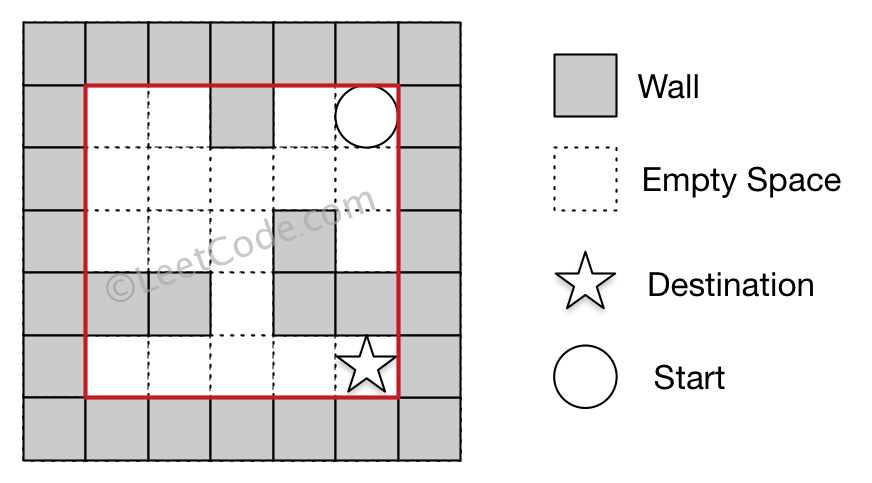
\includegraphics[width=150pt]{maze11.png}\\
\end{center}

\textbf{Example 2}

\textbf{Input 1:} a maze represented by a 2D array

\begin{Code}
0 0 1 0 0
0 0 0 0 0
0 0 0 1 0
1 1 0 1 1
0 0 0 0 0
\end{Code}

\textbf{Input 2:} start coordinate (rowStart, colStart) = (0, 4)
\textbf{Input 3:} destination coordinate (rowDest, colDest) = (3, 2)

\textbf{Output:} false

\textbf{Explanation:} There is no way for the ball to stop at the destination.

\begin{center}
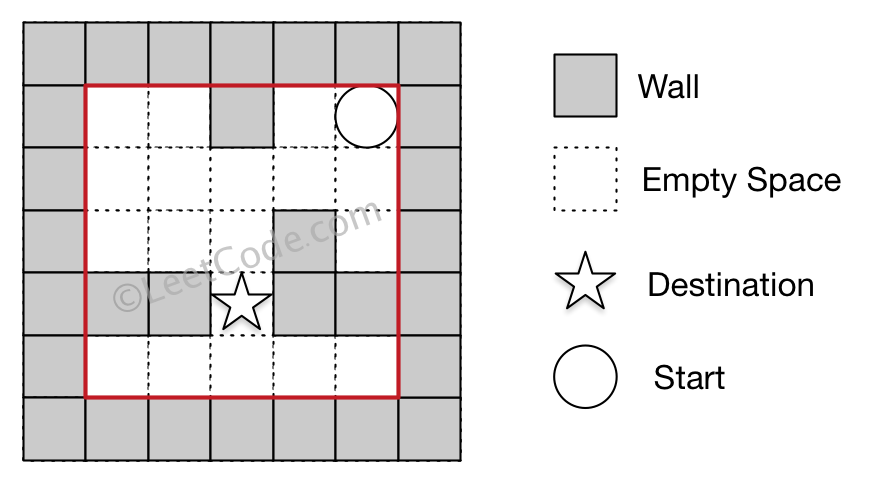
\includegraphics[width=150pt]{maze12.png}\\
\end{center}

\textbf{Note:}

1. There is only one ball and one destination in the maze.

2. Both the ball and the destination exist on an empty space, and they will not be at the same position initially.

3. The given maze does not contain border (like the red rectangle in the example pictures), but you could assume the border of the maze are all walls.

4. The maze contains at least 2 empty spaces, and both the width and height of the maze won't exceed 100.

\subsubsection{Solution}

\begin{Code}
public boolean hasPath(int[][] maze, int[] start, int[] destination) {

}
\end{Code}

\newpage

\section{The Maze II} %%%%%%%%%%%%%%%%%%%%%%

\subsubsection{Description}

There is a ball in a maze with empty spaces and walls. The ball can go through empty spaces by rolling up, down, left or right, but it won't stop rolling until hitting a wall. When the ball stops, it could choose the next direction.

Given the ball's start position, the destination and the maze, find the shortest distance for the ball to stop at the destination. The distance is defined by the number of empty spaces traveled by the ball from the start position (excluded) to the destination (included). If the ball cannot stop at the destination, return -1.

The maze is represented by a binary 2D array. 1 means the wall and 0 means the empty space. You may assume that the borders of the maze are all walls. The start and destination coordinates are represented by row and column indexes.

\textbf{Example 1}

\textbf{Input 1:} a maze represented by a 2D array
\begin{Code}
0 0 1 0 0
0 0 0 0 0
0 0 0 1 0
1 1 0 1 1
0 0 0 0 0
\end{Code}

\textbf{Input 2:} start coordinate (rowStart, colStart) = (0, 4)

\textbf{Input 3:} destination coordinate (rowDest, colDest) = (4, 4)

\textbf{Output:} 12

\textbf{Explanation:} One shortest way is : left -> down -> left -> down -> right -> down -> right.
             The total distance is 1 + 1 + 3 + 1 + 2 + 2 + 2 = 12.

\begin{center}
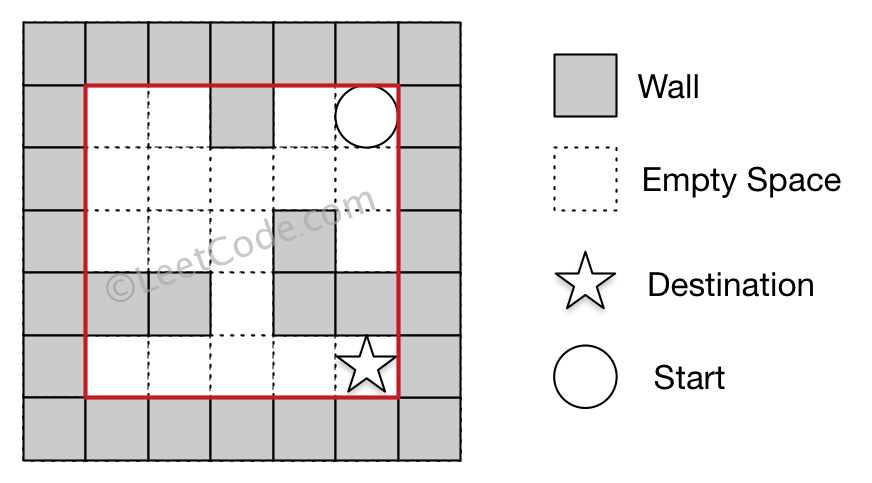
\includegraphics[width=150pt]{maze21.png}\\
\end{center}

\textbf{Example 2}

\textbf{Input 1:} a maze represented by a 2D array
\begin{Code}
0 0 1 0 0
0 0 0 0 0
0 0 0 1 0
1 1 0 1 1
0 0 0 0 0
\end{Code}

\textbf{Input 2:} start coordinate (rowStart, colStart) = (0, 4)

\textbf{Input 3:} destination coordinate (rowDest, colDest) = (3, 2)

\textbf{Output:} -1

\textbf{Explanation:} There is no way for the ball to stop at the destination.

\begin{center}
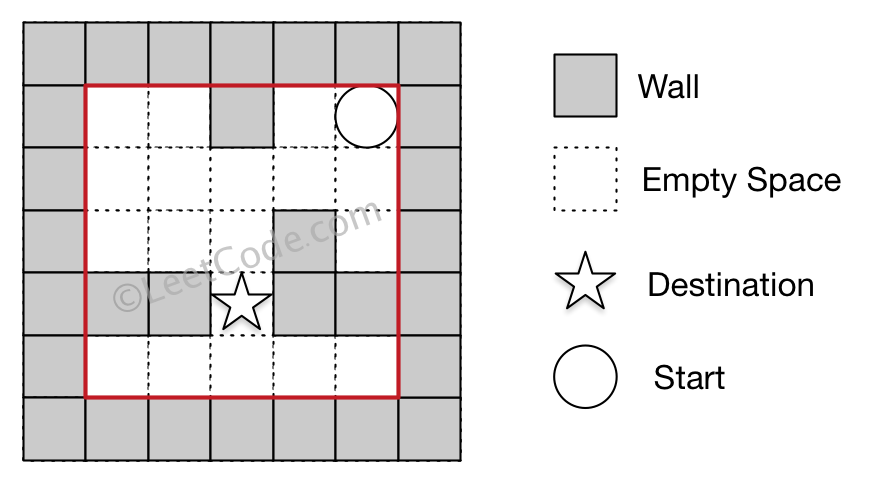
\includegraphics[width=150pt]{maze22.png}\\
\end{center}

\textbf{Note:}

1. There is only one ball and one destination in the maze.

2. Both the ball and the destination exist on an empty space, and they will not be at the same position initially.

3. The given maze does not contain border (like the red rectangle in the example pictures), but you could assume the border of the maze are all walls.

4. The maze contains at least 2 empty spaces, and both the width and height of the maze won't exceed 100.

\subsubsection{Solution}

\begin{Code}
public int shortestDistance(int[][] maze, int[] start, int[] destination) {

}
\end{Code}

\newpage

\section{The Maze III} %%%%%%%%%%%%%%%%%%%%%%

\subsubsection{Description}

There is a ball in a maze with empty spaces and walls. The ball can go through empty spaces by rolling up (u), down (d), left (l) or right (r), but it won't stop rolling until hitting a wall. When the ball stops, it could choose the next direction. There is also a hole in this maze. The ball will drop into the hole if it rolls on to the hole.

Given the ball position, the hole position and the maze, find out how the ball could drop into the hole by moving the shortest distance. The distance is defined by the number of empty spaces traveled by the ball from the start position (excluded) to the hole (included). Output the moving directions by using 'u', 'd', 'l' and 'r'. Since there could be several different shortest ways, you should output the lexicographically smallest way. If the ball cannot reach the hole, output "impossible".

The maze is represented by a binary 2D array. 1 means the wall and 0 means the empty space. You may assume that the borders of the maze are all walls. The ball and the hole coordinates are represented by row and column indexes.

\textbf{Example 1}

\textbf{Input 1:} a maze represented by a 2D array
\begin{Code}
0 0 0 0 0
1 1 0 0 1
0 0 0 0 0
0 1 0 0 1
0 1 0 0 0
\end{Code}

\textbf{Input 2:} ball coordinate (rowBall, colBall) = (4, 3)

\textbf{Input 3:} hole coordinate (rowHole, colHole) = (0, 1)

\textbf{Output:} "lul"

\textbf{Explanation:} There are two shortest ways for the ball to drop into the hole.

\begin{center}
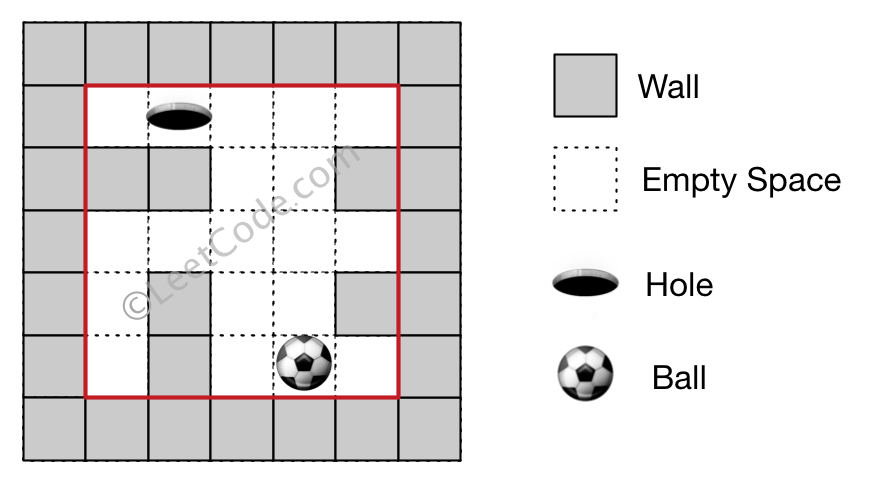
\includegraphics[width=150pt]{maze31.png}\\
\end{center}

The first way is left -> up -> left, represented by "lul".

The second way is up -> left, represented by 'ul'.

Both ways have shortest distance 6, but the first way is lexicographically smaller because 'l' < 'u'. So the output is "lul".

\textbf{Example 2}

\textbf{Input 1:} a maze represented by a 2D array
\begin{Code}
0 0 0 0 0
1 1 0 0 1
0 0 0 0 0
0 1 0 0 1
0 1 0 0 0
\end{Code}

\textbf{Input 2:} ball coordinate (rowBall, colBall) = (4, 3)

\textbf{Input 3:} hole coordinate (rowHole, colHole) = (3, 0)

\textbf{Output:} "impossible"

\textbf{Explanation:} The ball cannot reach the hole.

\begin{center}
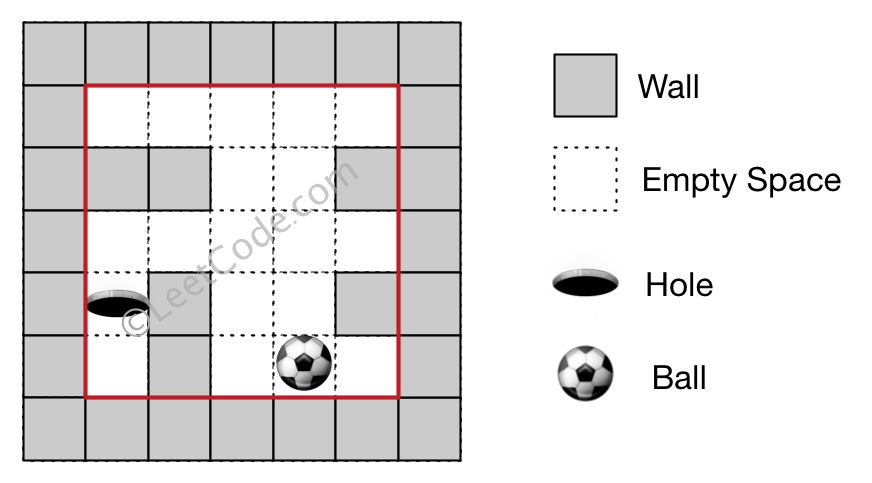
\includegraphics[width=150pt]{maze32.png}\\
\end{center}

\textbf{Note:}

1. There is only one ball and one hole in the maze.

2. Both the ball and hole exist on an empty space, and they will not be at the same position initially.

3. The given maze does not contain border (like the red rectangle in the example pictures), but you could assume the border of the maze are all walls.

4. The maze contains at least 2 empty spaces, and the width and the height of the maze won't exceed 30.

\subsubsection{Solution}

\begin{Code}
public String findShortestWay(int[][] maze, int[] ball, int[] hole) {

}
\end{Code}

\newpage

\section{01 Matrix} %%%%%%%%%%%%%%%%%%%%%%

\subsubsection{Description}

Given a matrix consists of 0 and 1, find the distance of the nearest 0 for each cell.

The distance between two adjacent cells is 1.

\textbf{Example 1:}

\textbf{Input:}
\begin{Code}
0 0 0
0 1 0
0 0 0
\end{Code}

\textbf{Output:}
\begin{Code}
0 0 0
0 1 0
0 0 0
\end{Code}

\textbf{Example 2:}

\textbf{Input:}
\begin{Code}
0 0 0
0 1 0
1 1 1
\end{Code}

\textbf{Output:}
\begin{Code}
0 0 0
0 1 0
1 2 1
\end{Code}

\textbf{Note:}

1. The number of elements of the given matrix will not exceed 10,000.

2. There are at least one 0 in the given matrix.

3. The cells are adjacent in only four directions: up, down, left and right.

\subsubsection{Solution}

\begin{Code}
public int[][] updateMatrix(int[][] matrix) {

}
\end{Code}

\newpage

\section{Lonely Pixel I} %%%%%%%%%%%%%%%%%%%%%%

\subsubsection{Description}

Given a picture consisting of black and white pixels, find the number of black lonely pixels.

The picture is represented by a 2D char array consisting of 'B' and 'W', which means black and white pixels respectively.

A black lonely pixel is character 'B' that located at a specific position where the same row and same column don't have any other black pixels.

\textbf{Example:}

\textbf{Input:}

\begin{Code}
[['W', 'W', 'B'],
 ['W', 'B', 'W'],
 ['B', 'W', 'W']]
\end{Code}

\textbf{Output: 3}

\textbf{Explanation:} All the three 'B's are black lonely pixels.

\textbf{Note:}

The range of width and height of the input 2D array is [1,500].

\subsubsection{Solution}

\begin{Code}
public int findLonelyPixel(char[][] picture) {

}
\end{Code}

\newpage

\section{Lonely Pixel II} %%%%%%%%%%%%%%%%%%%%%%

\subsubsection{Description}

Given a picture consisting of black and white pixels, and a positive integer N, find the number of black pixels located at some specific row R and column C that align with all the following rules:

Row R and column C both contain exactly N black pixels.

For all rows that have a black pixel at column C, they should be exactly the same as row R

The picture is represented by a 2D char array consisting of 'B' and 'W', which means black and white pixels respectively.

\textbf{Example:}

\textbf{Input:}
\begin{Code}
[['W', 'B', 'W', 'B', 'B', 'W'],
 ['W', 'B', 'W', 'B', 'B', 'W'],
 ['W', 'B', 'W', 'B', 'B', 'W'],
 ['W', 'W', 'B', 'W', 'B', 'W']]
\end{Code}

N = 3

\textbf{Output: 6}

\textbf{Explanation:} All the bold 'B' are the black pixels we need (all 'B's at column 1 and 3).
\begin{Code}
        0    1    2    3    4    5         column index
0    [['W', 'B', 'W', 'B', 'B', 'W'],
1     ['W', 'B', 'W', 'B', 'B', 'W'],
2     ['W', 'B', 'W', 'B', 'B', 'W'],
3     ['W', 'W', 'B', 'W', 'B', 'W']]
row index
\end{Code}

Take 'B' at row R = 0 and column C = 1 as an example:

Rule 1, row R = 0 and column C = 1 both have exactly N = 3 black pixels.

Rule 2, the rows have black pixel at column C = 1 are row 0, row 1 and row 2. They are exactly the same as row R = 0.

\textbf{Note:}

1. The range of width and height of the input 2D array is [1,200].

\subsubsection{Solution}

\begin{Code}
public int findBlackPixel(char[][] picture, int N) {

}
\end{Code}

\newpage